% header
\documentclass[10pt,a4paper]{article}

\usepackage[utf8]{inputenc}
\usepackage{hyperref}
\usepackage{amssymb}
\usepackage{amsthm}
\usepackage{amsmath}
\usepackage{ngerman}
\usepackage{gensymb}
\usepackage{enumitem}
\usepackage{graphicx}
\usepackage{stmaryrd}
\usepackage{listings}

\usepackage[]{algorithm2e}

%für pseudocode:
\SetKwProg{Fn}{Function}{}{end}\SetKwFunction{FRecurs}{FnRecursive}%
\SetAlgoLongEnd

%für argmax:
\newcommand{\argmax}{\operatornamewithlimits{argmax}}

%für folgepfeile mit begründung:
\newcommand{\MyArrow}{\operatornamewithlimits{\Rightarrow}}

%Das brauchen wir:
\newcommand{\zz}{\mathrm{Z\kern-.3em\raise-0.5ex\hbox{Z}}}

% the document
\begin{document}

% create the title
\title{Klausuraufgaben \\
\small{Kapitel 8 - Algorithmen auf Graphen}}
\author{Tom Kneiphof}
\date{\today}
\maketitle

\section*{Aufgabe 1}

\paragraph{a)}
Ein Matching $M \subseteq E$ eines ungerichteten Graphens $G = (V, E)$ ist eine Teilmenge der Kanten, so dass kein Knoten an zwei Kanten beteiligt ist.
\begin{equation*}
\forall \{v,w\}, \{x, y\} \in M \subseteq E : \{v, w\} \cap \{x, y\} = \emptyset
\end{equation*}


\paragraph{b)}
Bei einem \textbf{Nicht erweiterbaren Matching} handelt es sich um ein Matching $M$, zu dem keine Kante aus $E$ hinzugenommen werden kann, so dass es ein Matching bleibt.
\begin{equation*}
\forall \{v, w\} \in E \setminus M : M \cup \{ \; \{v, w\} \; \} \; \textnormal{ist kein Matching}
\end{equation*}

Bei einem \textbf{Maximales Matching} handelt es sich um ein Matching $M_{max}$ maximaler Gr\"o{\ss}e.
Es gibt also kein Matching welches mehr Kanten enth\"alt als $M_{max}$. Es gilt:
\begin{equation*}
\forall M : | M | \leq | M_{max} |
\end{equation*}


\paragraph{c)}
Satz von Berge: Ein Matching $M$ ist genau dann maximal, falls es keinen $M$-augmentierenden Pfad gibt.

\paragraph{d)}
Beweis des Satzes von Berge:

\paragraph{$\Rightarrow$}
Annahme: Es existiert ein $M$-augmentierender Pfad $P$.
Definiere $M' := M \oplus P$. Dann gilt $|M'| > |M|$, da $n$ Kanten entfernt wurden und $n+1$ Kanten hinzugef\"ugt wurden.
Dies ist ein Widerspruch dazu, dass $M$ bereits ein Maximales Matching war.

\paragraph{$\Leftarrow$}
Sei $M$ ein Matching in $G$, und existiere kein $M$-augmentierender Pfad. Sei weiter $M_{max}$ ein beliebiges maximales Matching in $G$. Annahme: $|M| < |M_{max}|$.
Betrachte $G' := (V, M \oplus M_{max})$. Da aus beiden Matchings je h\"ochstens eine Kante inzident zu $v$ sein kann, gilt:
\begin{equation*}
\forall v \in V : deg_{G'}(v) \leq 2
\end{equation*}
Die Zusammenhangskomponenten von $G'$ sind also isolierte Knoten, Kreise gerader L\"ange mit abwechselnden Kanten aus $M$ und $M_{max}$ oder Pfade mit abwechselnden Kanten aus $M$ und $M_{max}$.
Da $|M| < |M_{max}|$ angenommen wurde, gibt es einen $M$-augmentierenden Pfad $P$ in $G'$, dessen Endknoten beide $M$-frei sind. Da $P$ auch in $G$ existiert, gibt es einen $M$-augmentierenden Pfad in $G$, was ein Widerspruch dazu ist, dass ein solcher Pfad nicht existiert.

\section*{Aufgabe 2}
% Transformiere Nach erreichbarkeit in G_m
% + korrektheit
Gegeben sei ein Bipartiter Graph $G = (A, B, E)$ sowie ein Matching $M$ auf $G$. Konstruiere gerichteten Graphen $G_M = (A', B', E')$ wie folgt:
\begin{equation*}
A' := A \cup \{s\}  \qquad B':=B \cup \{t\} \qquad s,t \notin A \cup B \qquad s \neq t
\end{equation*}
Die Kanten die im Matching sind, werden von $A$ nach $B$ gerichtet und die Katen die nicht im Matching sind von $B$ nach $A$ gerichtet. Von $s$ aus sind die Knoten erreichbar die in $B$ $M$-frei sind, und von $M$-freien Knoten in $A$ aus ist $t$ erreichbar.
\begin{equation*}
E_1 := \{ \, (u, v) \mid (u, v) \in M, u \in A, v \in B \, \} \\
\end{equation*}
\begin{equation*}
E_2 := \{ \, (u, v) \mid (u, v) \in E \setminus M, u \in B, v \in A \, \}
\end{equation*}
\begin{equation*}
E_3 := \{ \, (s, b) \mid b \in B \textnormal{ ist $M$-frei} \, \} \cup \{ \, (a, t) \mid a \in A \textnormal{ ist $M$-frei} \, \}
\end{equation*}
\begin{equation*}
E' := E_1 \cup E_2 \cup E_3
\end{equation*}
Nun existiert in $G_M$ genau dann ein Pfad von $s$ nach $t$, wenn ein $M$-augmentierender Pfad in $G$ existiert.
\paragraph{Beweis}

\paragraph{$\Rightarrow$}
Sei $P = s, v_0, \ldots, v_k, t$ ein Pfad von $s$ nach $t$ in $G_M$.
Daraus folgt direkt, dass $v_0 \in B$ $M$-frei ist, sowie $v_k \in A$ $M$-frei.
Aus der Konstruktion von $E'$ folgt, dass die Kanten $(v_i, v_{i+1})$ abwechselnd aus $M$ und $E \setminus M$ kommen.
Also ist $v_0, \ldots, v_k$ ein $M$-augmentierender Pfad in $G$.

\paragraph{$\Leftarrow$}
Sei $P = v_0, \ldots, v_k$ ein $M$-augmentierender Pfad in $G$. O.B.d.A. seien $v_0 \in B$ und $v_k \in A$.
\begin{enumerate}
	\item $(s, v_0) \in E'$ da $v_0$ $M$-frei ist, und $v_0 \in B$
	\item $(v_k, t) \in E'$ da $v_k$ $M$-frei ist, und $v_k \in A$
	\item $v_i \in A$ falls $i$ ungerade
	\item $v_i \in B$ falls $i$ gerade
	\item $\{v_i, v_{i+1}\} \in M$ falls $i$ ungerade
	\item $\{v_i, v_{i+1}\} \in E \setminus M$ falls $i$ gerade
\end{enumerate}
Es existiert also eine Kante $(s, v_0) \in E'$ und $(v_k, t) \in E'$,
sowie die Kanten $(v_i, v_{i+1}) \in E'$.
Damit ist $P' = s, v_0, \ldots, v_k, t $ ein Pfad von $s$ nach $t$ in $G_M$.


\section*{Aufgabe 3}
    
    Kurz und anschaulich: \\
    wir haben bipartiten Graphen und führen auf jedem
    Knoten der Seite am ``Quellknoten'' Tiefensuche aus \\
    $\Rightarrow O(|V| \cdot (|V| + |E|))$
    

\section*{Aufgabe 4}

    \begin{enumerate}[label={\alph*)}]
        \item Ein gültiges Matching ist eine Menge $M \subseteq E$ wenn keine
            zwei unterschiedliche Elemente aus $M$ einen gemeinsamen Knoten
            haben.
            Ein Matching $M'$ heißt nicht erweiterbar, wenn es keine Kante
            $ e \in E \setminus M$ gibt, sodass $\{e\} \cup M$ ein gültiges
            Matching ist.
        \item
            \textbf{Algo:}\\
            \begin{algorithm}[H]
                
                \Fn{GenM(G = (V,E))}{
                    V' := V\;
                    M := $\emptyset$\;
                    \For{$e = (u,v) \in E$} {
                        \If{$u,v \in V'$}{
                            $M := M \cup \{ e \}$\;
                            $V' := V' \setminus \{x,y\}$\;
                        }
                    }
                }
                
            \end{algorithm}

        \item
            $\zz$: $M$ ist nicht erweiterbares Matching $\Rightarrow
            |M| \geq \frac{1}{2}|M_{max}|$
            \\
            \textbf{Annahme:} $M$ ist nicht erweiterbares Matching und
            $|M| < \frac{1}{2}|M_{max}|$
            \\
            Dann muss es aber eine Kante $m_0 \in M_{max}$ geben für
            die gilt: $m_0 \notin M$ und die Kante Verbindet zwei Knoten,
            die von keiner Kante in $M$ überdeckt werden
            \\
            $\Rightarrow M$ kann um $m_0$ erweitert werden
            \\
            $\Rightarrow M$ ist nicht ein nicht erweiterbares Matching
            $\lightning$ Widerspruch!
        \item

    \end{enumerate}

\section*{Aufgabe 05}

    \begin{enumerate}[label={\alph*)}]
    
    \item \textbf{Algo:} \\
        
        \begin{algorithm}[H]
        
            \Fn{IsBipartit($G = (V,E)$)}{
            
                \For{$v \in V$}{
                    $color(v ) := 0$\;
                }
                $V' := V$\;
                \While{ $V' \neq \emptyset$ }{
                    $s = $ zufälliger Knoten aus $V$\;
                    \If{not Mod\_DFS(s,-1, $V'$)}{
                        return false\;
                    }
                    
                }
                return true\;
            }
            
            \Fn{Mod\_DFS(v, prevColor, $V'$)}{
                $color(v) = prevColor * (-1)$\;
                $V' \setminus \{v\}$\;
                \For{$(v,u) \in E $}{
                    \If{color(u) == color(v)}{
                        return false\;
                    }
                    \ElseIf{color(u) == 0}{
                        \If{not Mod\_DFS(u,color(v), $V'$)}{
                            return false\;
                        }
                    }
                }
                return true\;
            }
        
        \end{algorithm}
        
        
    \item
    
        selber Algo wie in a), nur für jede Kante einmal mit ohne diese Kante
        \\$\Rightarrow O(|E| \cdot (|V| + |E|))$
        
    \end{enumerate}
    
    
\section*{Aufgabe 06}

    \textbf{Beweise den Satz von König:} \\
    Sei $G = (V,E)$ ein bipartiter Graph und $V$ ist unterteilt in
    die Mengen $L$ und $R$. Sei $M$ ein maximales Matching für $G$.
    Da kein Knoten einer Knotenüberdeckung mehr als eine Kante von $M$
    überdecken kann, muss eine Knotenüberdeckung mit $|M|$ Knoten eine
    maximale Knotenüberdeckung sein.
    \\
    \textbf{Zeige, dass eine solche Überdeckung konstruiert werden kann:}
    \\
    Sei $U$ die Menge der ungematchten Knoten in $L$ und sei $Z$ die Menge
    der Knoten die entweder in $U$ selber sind, oder durch alternierende Pfade mit
    Knoten in $U$ verbunden sind. Ferner sei
    $$
        K = (L\setminus Z) \cup (R\cap Z)
    $$
    jede Kante $e$ in $G$ erfüllt eine der folgenden Bedingungen:
    \begin{itemize}
        \item[a)] $e$ ist Teil eines alternierenden Pfades (und hat einen ``rechten''
        Endpunkt in $K$)
        \item[b)] $e$ hat einen ``linken'' Endpunkt in $K$
    \end{itemize}
    Für den Fall, dass $e$ gematched aber nicht in einem alternierenden Pfad ist, gilt:
    dass der linke Endpunkt nicht in einem alternierenden Pfad sein kann und in $L\setminus Z$
    enthalten ist. Für den Fall, dass $e$ nicht gematched ist und nicht in
    einem alternierenden Pfad ist gilt: der linke Endpunkt  kann ebenfalls nicht in
    in einem alternierenden Pfad sein (denn dieser könnte durch $e$ erweitert werden).
   \\
   Ebenso gilt: jeder Knoten $k \in K$ ist ein Endpunkt von einer gematchten
   Kante, da gilt:
   \begin{itemize}
        \item  falls $k \in L\setminus Z $: $k $ist gematched, da $Z$ eine Obermenge von $U$ ist.
        \item falls $k \in R\cap Z$: $k$ ist gematched, da k Teil eines alternierenden
            Pfades ist (und  nicht der Endpunkt des alternierenden Pfades sein kann)

   \end{itemize}
    Letztendlich kann also keine Kante beide Endpunkte in $K$ haben
    $\Rightarrow$ K ist eine Knotenüberdeckungen mit $|K| = |M|$ und $K$ muss
    eine minimale Knotenüberdeckung sein.

\section*{Aufgabe 07}

	$\zz$: für alle $u,v, \in V$ mit $num(u) > num(v)$ gilt:\\
	$\exists$ Pfad $P$ von $v$ nach $u$ mit $num(w) \leq num(u) \forall w$
	auf $P \Rightarrow u$ und $v$ sind in der selben Zusammenhangskomponente
	\\
	\textbf{Beweis:}\\
	Damit $u$ und $v$ in der selben Zusammenghangskomponente sind, muss gelten:
	\begin{enumerate}[label={\alph*.}]
		\item
			$\exists$ Pfad von $u$ nach $v$
		\item
			$\exists$ Pfad von $v$ nach $u$
	\end{enumerate}
	Die zweite Bedingung ist durch die Aufgabenstellung erfüllt. Bleibt zu zeigen:
	$\exists$ Pfad von $u$ nach $v$. \textbf{Annahme:} $\nexists$
	Pfad von $u$ nach $v \Rightarrow$ $v$ kann kein Knoten im Teilbaum mit
	Wurzel $u$ (im Tiefensuche Baum) sein. Betrachte den Pfad:
	$$
		P = [v = w_1, \ldots, w_k = u]
	$$
	Zudem gilt: offensichtlich kann die Tiefensuche beim Betreten des Knotens $v$
	den Knoten $u$ noch nicht betrachtet haben (weil $num(u) > num(v)$).
	Betrachte nun den Knoten $w_i$ (evtl. auch $w_1$), der beim Betreten von $v$ schon betrachtet
	wurde und am nächsten zu u liegt (also den Knoten mit maximalem i,für den diese
	Bedingung gilt). Dieses i muss kleiner $k$ sein ($w_K = u$ ist unbetrachtet).
	Dann können folgende Fälle auftreten:
	\begin{itemize}
		\item $w_i$ ist nicht im Tiefensuche-Keller
			$\Rightarrow w_i$ ist fertig abgearbeitet und wurde aus
			dem Stack entfernt \\
			$\Rightarrow $ alle Kindknoten von $w_i$ wurden bereits betrachtet\\
			$\Rightarrow w_{i+1}$ wurde auch schon betrachtet.\\
			$\Rightarrow i$ war nicht maximal gewählt $\lightning$
		\item $w_i$ ist im Tiefensuche Keller \\
			$\Rightarrow u$ muss in einem Teilbaum mit Wurzel $v$ sein (sonst wäre für das maximale $w_i$
				der obere Fall eingetreten)\\
			$\Rightarrow num(v) > num(u) \lightning$
	\end{itemize}
	$\Rightarrow$ Annahme kann nicht zutreffen \hfill $\qed$

\section*{Aufgabe 08}

	\begin{enumerate}[label={\alph*)}]

		\item
			\textbf{Definition reduzierter Graph}: \\
			$G'_{red} = (V_{red},E_{red})$ mit
			\begin{itemize}
				\item
					jeder Knoten $v_{i} \in V_{red}$ steht für eine
					Zusammenhangskomponente $G'_i=(V_i,E_i)$
					$\Rightarrow \forall v,u \in V_{red}, v \neq u : 
					\neg(\exists $ Pfad von $ u $ nach $v \wedge \exists $ Pfad von $v$ nach $u$ )
				\item
					$(v_i,v_j) \in E_{red} \Leftrightarrow \exists u_i \in V_i,
						u_j \in V_j: (u_i,u_j) \in E'$
			\end{itemize}

		\item
		\textbf{Beweis} (aus dem Buch) : \\
		(\textbf{R}) $\Rightarrow$ Für alle Knoten $v$ die während der Tiefensuche
			auf G' mit Startknoten $u$ besucht werden gilt: $\exists$ Pfad P in G von
			$v$ nach $u$ mit $num(w) \leq num(u) \forall w$ auf P. Dann gibt es zwei Fälle:
			\begin{itemize}
				\item
					$num(u) > num(v) \Rightarrow u$ und $v$ sind in der selben Zusammenhangskomponente
					(siehe voherige Aufgabe).
				\item
					$num(u) \leq num(v) \Rightarrow $ nach (\textbf{R}) wurde die Komponente
						die $u$ enthält bereits konstruiert.
			\end{itemize}

	\end{enumerate}
	

\section*{Aufgabe 09}

    \textbf{Textiuelle Beschreibung des Graphen:} \\
    
    \begin{itemize}
        \item Führe auf Graph G Tiefensuche aus und nummeriere besuchte Knoten aufsteigend durch num(v)
        \item transponiere Graph: $G’ := V, E’$ mit $E’ = e \in E :(w,v)$ ist$ (v,w) \in E'$
        \item Sortiere $v \in V$ nach $n(v_i)_{max}>\ldots>num(v_j)_{min}$
        \item Führe Tiefensuche aus, s.d. nur noch nicht betrachtete Knoten betrachtet werden
        \item Füge alle mit dieser Tiefensuche erreichten Knoten in eine ZHK und markiere sie als betrachtet
        \item Gehe zu nächst höchstem noch nicht betrachteten Knoten, falls noch nicht alle Knoten betrachtet
        
    \end{itemize}

\section*{Aufgabe 10}


    \textbf{Kante in einem Graphen löschen:}
    \begin{itemize}
    
    \item Kante spielt ist kein Element einer SZK. $\rightarrow$ Anzahl ändert sich nicht
    \item Kante ist in einem Graph von |V|,|E|=n, die auf einem Kreis liegen und so eine SZK. bestehend aus n Knoten bilden. wenn jetzt eine Kante Gelöscht wird bricht diese SZK. auf und es existieren nurnoch ein-elementige SZK. Wir haben dann n SZK. also n-1 mehr SZKs. als vorher.
    \end{itemize}
    
    \textbf{Kante in einem Graphen hinzufügen:}
    
    \begin{itemize}
    
    \item Kante spielt keine Rolle, es entsteht keine veränderung der SZKs. $\rightarrow$ Anzahl ändert sich nicht.
    \item Kante schließt eine linerare Verkettung von n Knoten von letzten auf ersten Knoten, s.d. ein Kreis entsteht, die vorher n SZKs werden zu einer $\rightarrow$ Die Anzahl verringert sich um n-1 SZKs.
        
    \end{itemize}

\section*{Aufgabe 11}

	\begin{enumerate}[label={\alph*)}]
		\item
			$\zz: G_{szk}$ ist azyklisch\\
			\textbf{Annahme:} $G_{szk}$ ist nicht azyklisch \\
			$\Rightarrow \exists $ Kreis in $G_{szk}$ \\
			$\Rightarrow \exists v_i \in V_{szk}, v_j \in V_{szk}: \exists $
			Pfad von $v_i$ nach $v_j$ und umgekehrt in $G_{szk}$ \\
			$\Rightarrow \forall $ Knoten $u_i$ bzw. $u_j$ die in der zur $v_i$ bzw $v_j$
				korrespondierenden SZK sind gilt: $\exists $ Pfad von $u_i$ nach $u_j$ und
				umgekehrt in G. \\
			$\Rightarrow u_i $ und $u_j$ müssen sich in der selben starken zusammenhangskomponente
			befinden \\
			$\Rightarrow G_{szk}$ ist kein starker Zusammenhangskomponentengraph $\lightning$
		\item
			Vorgehensweise des algos:
			\textbf{Eingabe: } Graph $G=(V,E)$
			\\ \textbf{Ausgabe: } Graph $G_{szk} = (V_{szk}, E_{szk})$\\
			\begin{algorithm}[H]
				$V_{szk}$ := $\emptyset$\;
				$E_{szk}$ := $\emptyset$\;
				$V' $:= $V$\;
				$E'$ := $\{(v,u) | (u,v) \in E \} $\;
				$G' := (V,E')$ \;
				führe Erledigungsorientierte Nummerierung auf $G$ aus \;
				\While{$V' \neq \emptyset$}{
					$v' = \argmax\limits_{v'} \quad num(v') $ mit $v' \in V'$\; 
                    $V' \setminus \{ v' \}$ \; 
                    \textbullet erstelle neuen Knoten $v'_{szk}$ in $V_{szk}$ \;
                    \textbullet führe DFS auf $G'$ beginndend bei $v'$ durch mit modifikationen: \\
                    \begin{itemize}
                        \item merke für jeden besuchten Knoten, dass er mit $v'_{szk}$ korrespondiert.
                        \item findet DFS eine Kante zu einem Knoten $u$ mit $num(u) > num(v')$
                            wird eine Kante $(v'_{szk}, u'_{szk})$ zu $E_{szk}$ hinzugefügt (wobei $u'_{szk}$
                            der zu $u$ korrespondierende Knoten in $V_{szk}$ ist ). Anschließend verlasse
                            diesen Teilbaum.
                        \item entferne jeden besuchten Knoten v aus V' 
                    \end{itemize}
                    
				}
				return $G_{szk} =(V_{szk}, E_{szk})$
			\end{algorithm}
			
            \textbf{Korrektheit:} \\
            $\zz$ Ausgabe des Algos ist ein reduzierter Graph. \\
           $G'$ ist erledigungsorientiert durchnummeriert. \\
            \begin{itemize}
                \item
                 
                $\MyArrow\limits_{Aufgabe 8}$ modifizierte DFS erzeugt keine
                Kanten zu Knoten in $V{szk}$ die schon betrachtet wurden. \\
                $\Rightarrow G_{szk} $ ist azyklisch
                
                \item
                
                $\MyArrow\limits_{Aufgabe 7}$ alle durch modifizierte DFS gefundenen Knoten $U$
                für die gilt $num(u) < num(v')$ sind in der selben zusammenhangskomponente.
                
            \end{itemize}
            
            zusammen folgt daraus, dass der Algorithmus einen korrekten Komponentengraphen erstellt
           
            \item
            \textbf{textuelle Beschreibung des Algos:}: \\
            \begin{itemize}
                \item jage $G$ einmal durch den Algo aus $b)$ und speichere Ergebnis in $G'$
                \item \textbf{while} ($V' \neq \emptyset$):
                \begin{itemize}
                    \item \textbf{if} (\#Knoten mit Ingrad(0) $>$ 1):
                    \begin{itemize}
                        \item return \textbf{false}
                    \end{itemize}
                    \item entferne Knoten mit Ingrad(0) (und entsprechende Kanten)

                \end{itemize}
                
                return true

            \end{itemize}
            
            \textbf{Korrektheit:}
            och nööö

	\end{enumerate}

\section*{Aufgabe 12}

    \begin{itemize}
        \item   Einzelpaar-kürzeste-Weg-Problem (single-pair shortest-path problem oder
        single-source single-sink shortest-path problem): Gegeben $G = (V, E, w)$ und zwei
        Knoten $s,t \in V$ möchte man einen kürzesten Pfad von  $s$ nach $t$ finden.
        \item Einzelquelle-kürzeste-Weg-Problem (single-source shortest-path problem):
        Gegeben $G = (V, E, w)$ und einen (Quell-)Knoten $s \in V$, soll für jeden Knoten $v \in V$
        ein kürzester Pfad von $s$ zu $v$ gefunden werden.
        \item Alle-Paare-kürzeste-Weg-Problem (all-pairs shortest-path problem): Hier möchte
		man, gegeben $G = (V, E, w)$, für jedes Paar $u,v \in V$, einen kürzesten Pfad von u nach v
		finden.
	\end{itemize}

\section*{Aufgabe 13}
    \textbf{Annahme: } Sei $P$ ein kürzester Pfad und $\exists P_{ij}$
    wobei $P_{ij}$ nicht der kürzeste Pfad von $v_i$ nach $v_j$ ist.
    Dann folgt trivialerweise, dass es einen kürzeren Pfad $P'_{ij}$ gibt
    und einen Pfad $P' = v_1, \ldots, v_i, \ldots, v_j, \ldots, v_k$ mit
    $|P'| = |P| - (|P_{ij}| - |P'_{ij}|)$ \\ $\Rightarrow |P'| < |P|$
    \\ $\Rightarrow P$ ist nicht kürzester Pfad $\lightning$
    

\section*{Aufgabe15}

    TODO

\section*{Aufgabe 16}
    
    \begin{algorithm}[H]
     
     m := max(w) + 1 mit $0 < w < \infty$\;
     \For{$w \in W$}{
        $w = -w + m$\;
     }
     
    \end{algorithm}
    
    Dann dijkstra \ldots

\section*{Aufgabe 17}


    
\section*{Aufgabe 18}

    \begin{enumerate}[label={\alph*)}]
        \item 

            \textbf{Bellman-Ford-Algo}: \\
            \begin{algorithm}[H]
            \For{$v \in V$}{
                d(v) := $\infty$ \;
                $\pi(v)$ := \textbf{NULL} \;
            }
            d(s) := 0 \;
            \For{i \KwTo $|V|$ }{
                \For{ $(u,v) \in  E$ }{
                    \If{d(u) + w(u,v)  $<$ d(v)}{
                        d(v) :=d(u) + w(u,v) \;
                        $\pi(v)$ := u \;
                    }
                }
            }
            \For{$(u,v) \in E$}{
                \If{d(u) + w(u,v) $<$ d(v)}{
                    \#Zyklus mit negativem Gewicht \;
                    return ERROR \;
                }
            }
            
            return \{$(v,d(v)) | v \in V$\} \;
            \end{algorithm}
            
            \textbf{Komplexität:} Durch Betrachten der Schleifen offensichtlich  $O(|V| \cdot |E|)$            
            
        \item
            TODO: für mich ist die Definition von $d^l(j)$ aus der Vorlesung widersprüchlich
                $\Rightarrow $ frage im Ferientutorium.
            

    \end{enumerate}
    
    
    

\section*{Aufgabe 21}
	\paragraph{Annahme:} $(u,v)$ ist nicht sicher bzgl. $\tilde{A}$, also $(u, v) \notin A$.
	Konstruiere anderen überspannenden Baum $T' = (V, A', w)$ mit $\tilde{A} \cup \{(u,v)\} \subseteq A'$ wie folgt:

	Betrachte Pfad $P$ von $u$ nach $v$ in $T$. Dieser bildet zusammen mit $(u, v)$ einen Kreis.
	Da $(u,v)$ den Schnitt $(S, V \setminus S)$ kreuzt, existiert $(x, y) \in P$ so dass $(x, y)$ den Schnitt $(S, V \setminus S)$ kreuzt.
	Entfernt man $(x,y)$ aus $T$ und fügt $(u,v)$ ein, so erhält man den neuen überspannenden Baum $T'$
	mit $A' = A \setminus \{(x, y)\} \cup \{(u, v)\}$.
	Da $(u, v)$ eine Kandidatskante war, gilt $w(u,v) \leq w(x, y)$.
	\begin{equation*}
	w(T') = w(T) - w(x, y) + w(u,v) \leq w(T)
	\end{equation*}
	Da $T$ bereits ein minimaler überspannender Baum war, muss $w(T') = w(T)$ sein und $T'$ ist ein minimaler überspannender Baum.
	$(x, y) \notin \tilde{A}$, da $\tilde{A}$ den Schnitt $(S, V \setminus S)$ respektiert, $(x, y)$ diesen aber kreuzt.
	Also ist $\tilde{A} \subseteq A'$. $(u, v)$ sicher bzgl. $\tilde{A}$.

\section*{Aufgabe 22}
	\paragraph{Eingabe:} Ungerichteter, gewichteter Graph $G=(V, E, w)$
	\paragraph{Ausgabe:} Minimaler $G$ überspannender Spannwald $T=(V, A, w)$
	\begin{lstlisting}[language=Java]
A = new Set();
Q = new Array(E);
sort(Q, incr by w);
UF = makeUnionFind(V);
for ((u, v) in Q)
{
	idU = UF.find(u);
	idV = UF.find(v);
	if (idU != idV)
	{
		UF.union(idU, idV);
		A.insert((u, v));
	}
}
return T = (V, A, w);
	\end{lstlisting}


\section*{Aufgabe 23}
Sei $G = (V, E, w)$ ungerichteter, gewichteter Graph mit $\forall e_1, e_2 \in E : w(e_1) \neq w(e_2)$, $T = (V, A, w)$ minimaler überspannender Baum von G. $T$ existiert, da $G$ als zusammenhängend vorausgesetzt wird.
\paragraph{Wissen} Jeder minimale überspannende Baum $T$ von $G$ hat genau $|V|-1$ viele Kanten. Gäbe es weniger Kanten, gäbe es einen Knoten, der nicht mit dem Baum verbunden wäre, gäbe es mehr Kanten, so gäbe es einen Kreis.
\paragraph{}
Wähle eine beliebige Kante $(u, v) \in A$ und entferne diese. Damit T nun wieder ein überspannender Baum wird, muss eine geeignete Kante $(x, y) \in E \setminus \{(u,v)\}$ wieder hinzugefügt werden.
Sei $T' = (V, A', w)$ mit $A' = A \setminus \{(u,v)\} \cup \{(x,y)\}$.
Da alle Kanten unterschiedliche Gewichte haben, gilt $w(u,v) \neq w(x, y)$.
\begin{itemize}
	\item Falls $w(u, v) < w(x, y)$, so ist $w(T') > w(T)$ und T' kein minimaler überspannender Baum mehr.
	\item Falls $w(u, v) > w(x, y)$, so ist $w(T') < w(T)$, was ein widerspruch dazu ist, dass $T$ ein minimaler überspannender Baum war.
\end{itemize}

Also existiert genau ein minimaler überspannender Baum $T$ von $G$.

\section*{Aufgabe 24}

    okay, ich finde die Reihenfolge der Teilaufgaben leicht suboptimal,
    deshalb kommt die b zuerst ;) \\
    \begin{itemize}
        \item[b)]
            \begin{itemize}
            \item \textbf{Algo: } Prim \\
            \item \textbf{Eingabe: } zusammenhängender, gewichteter, ungerichteter Graph $G =(V,E,w)$ \\
            \item \textbf{Ausgabe} minimaler überspannender Baum $T = (V,A,w)$\\
            \item \textbf{implementierung: } \\
            
                \begin{algorithm}[H]
                    
                    $Q := V$\;
                    $s := Q.getRandomItem()$\;
                    $d(s) := 0$\;
                    $\pi (s):= null$\;
                    \For{$u \in Q \setminus \{s\}$}{
                        $d(u) := \infty$\;
                    }
                    \While{$Q \neq \emptyset$}{
                        $u := {argmin}_u (d(u)), u \in Q$ \;
                        $Q := Q \setminus \{u\}$ \;
                        \For{$(u,v) \in E$}{
                            \If{$v \in Q$ \textbf{and} $w(u,v) < d(v)$ } {
                                $d(v) := w(u,v)$ \;
                                $\pi (v) := u$ \;
                            }
                        }
                    }
                    
                    $A := \emptyset$\;
                    \For{$ v \in V$}{
                        \If{$\pi (v) \neq null$}{
                            $A.append((\pi (v), v))$\;
                        }
                    }
                    
                    \textbf{return} $T = (V,A,w)$ \;
                
                \end{algorithm}

            
            \end{itemize}
            
            \item[a)]
                \textbf{Korrektheit:} (frei nach der englischen Wikipedia)\\
                    Sei $G$ ein zusammenhängender gewichteter Graph.
                    Bei jedem Schleifendurchlauf wird eine Kante gefunden, die einen
                    Knoten, der noch nicht in $T$ liegt mit $T$ verbindet.
                    Da $G$ zusammenhängend ist gibt es immer einen Pfad zwischen
                    zwei beliebigen Knoten. Die Ausgabe des Algos muss ein Baum sein,
                    da jeder Knoten max. einen Vorgänger hat und die dazu korrespondierende
                    Kante hinzugefügt wurde.\\
                    
                    \textbf{Anmerkung zu folgenden Beweis: } 
                    Die Folgepfeile dienen eher der Strukturierung des textuell geführten Beweises
                    und sind nicht zwingend als Aussagenlogisch einwandfreie Folgerungen zu verstehen :P\\
                    
                    Sei nun $T_{min}$ ein minimaler Überspannder Baum von $G$.\\
                    $\zz: \quad T = T_{min}$\\
                    \textbf{Annahme:} $T > T_{min}$ \\
                    Dann sei $e$ die erste Kante, die zu $T$, nicht aber zu $T_{min}$ hinzugefügt wurde,
                    und V' sei die Menge der verbundenen Knoten, bevor $e$ hinzugefügt wurde.
                    \\ $\Rightarrow$ Ein Endpunkt von $e$ ist in V', der andere nicht.
                    \\ Da $T_{min}$ minimaler Spannbaum ist, muss ein Pfad darin existieren,
                    der eben jene Endpunkte miteinander verbindet. Damit muss dieser Pfad zusätzlich
                    eine Kante $f$ enthalten, die einen Knoten aus V' mit einem Knoten außerhalb
                    verbindet.
                    \\$\Rightarrow$ zum Zeitpunkt des betrachteten Iterationsschrittes
                    hätten wir also statt $e$ auch $f$ hinzunehmen können.
                    Da wir aber $f$ als mögliche Kante ausgeschlossen haben, muss gelten:
                    $w(f) \geq w(e)$. \\
                    Betrachte nun zusätzlich noch einen Baum $T_2$, der entsteht, wenn von
                    $T_{min}$ die Kante $f$ entfernt und anschließend $e$ hinzugefügt wird.
                    \\ $\Rightarrow T_2$ ist offensichtlich zusammenhängend, hat die selbe Knotenanzahl
                    wie $T_{min}$ und die Summe der Kantengewichte ist nicht größer als die von $T_{min}$
                    \\ $\Rightarrow T_2$ ist ebenfalls ein minimaler Spannbaum von $G$ und enthält
                    $e$ sowie alle Kanten, die vor dem betrachteten Iterationsschritt schon
                    hinzugefügt wurden. Führen wir nun den Algorithmus weiter mit diesem Teilergebnis
                    durch, (und wiederholen induktiv diese Schritte für jede Kante) bekommen wir einen
                    Spannbaum $T_2$ mit $T_2 = T \leq T_{min} \lightning$
                    \\
                    Damit haben wir $T > T_{min}$ widerlegt und gezeigt, dass die Ausgabe
                    $T$ ein minimaler Spannbaum sein muss
            
    \end{itemize}

\section*{Aufgabe 25}

    \begin{itemize}
        
        \item \textbf{Flussnetzwerk:}\\
        Sei $G = (V,E,c,s,t) $ mit Quelle $s \in  V$, Senke $t \in V \setminus \{s\}$ und
        Kapazitätsfunktion $c : E \rightarrow \mathbb{R}^+$, die jeder Kante $ e = (v,w)$ eine
        positive reellwertige Kapazität $c(v,w)$ zuordnet. Dann ist $G$ ein Flussnetzwerk.
        
        \item \textbf{Fluss:}\\
            ein Fluss $f : V \times V \rightarrow \mathbb{R}$ ist eine Funktion, die
            folgende Bedingung erfüllt:
            \begin{enumerate}
                \item \textbf{Kapazitätsbedingung:}
                    \\ $f(v,w) \leq c(v,w) $ für alle $(v,w) \in V \times V$
                    
                \item \textbf{Kirchhoffsches Gesetz:}
                    \\$\sum\limits_{e \in IN(v)} f(e) = \sum\limits_{e \in OUT(v)} f(e)$
                    für alle $v \in V \setminus \{s,t\} $
            \end{enumerate}
    
    \end{itemize}
    
            
\section*{Aufgabe 26}

    \textbf{Ansatz:} \\
    Gegeben sei ein bipartiter Graph $G = (L,R,E)$ . Füge Quelle $s$ und Senke $t$
    hinzu, und verbinde alle Knoten von L jeweils mit einer Kante mit Kantengewicht 1 mit s
    (gerichtet von s nach $l \in L$)und
    analog alle Knoten von R mit einer Kante mit Kantengewicht 1 mit t (gerichtet von $r \in R$ nach t).
    Gewichte zusätzlich alle Kanten in E mit 1 und richte sie aus, sodass alle
    Kanten in E die Form haben: $ (l,r), l\in L, r \in R$. Dann löse das maximale Flussproblem
    mit Quelle s und Senke t und merke Kanten zwischen L und R, die zum maximalen Fluss
    gehören. Diese Kanten bilden ein maximales Matching.

\section*{Aufgabe 27}

    Folgender Graph widerlegt beides:
     \begin{figure}[!htb]
        \centering
        \resizebox{0.8\textwidth}{!}{
            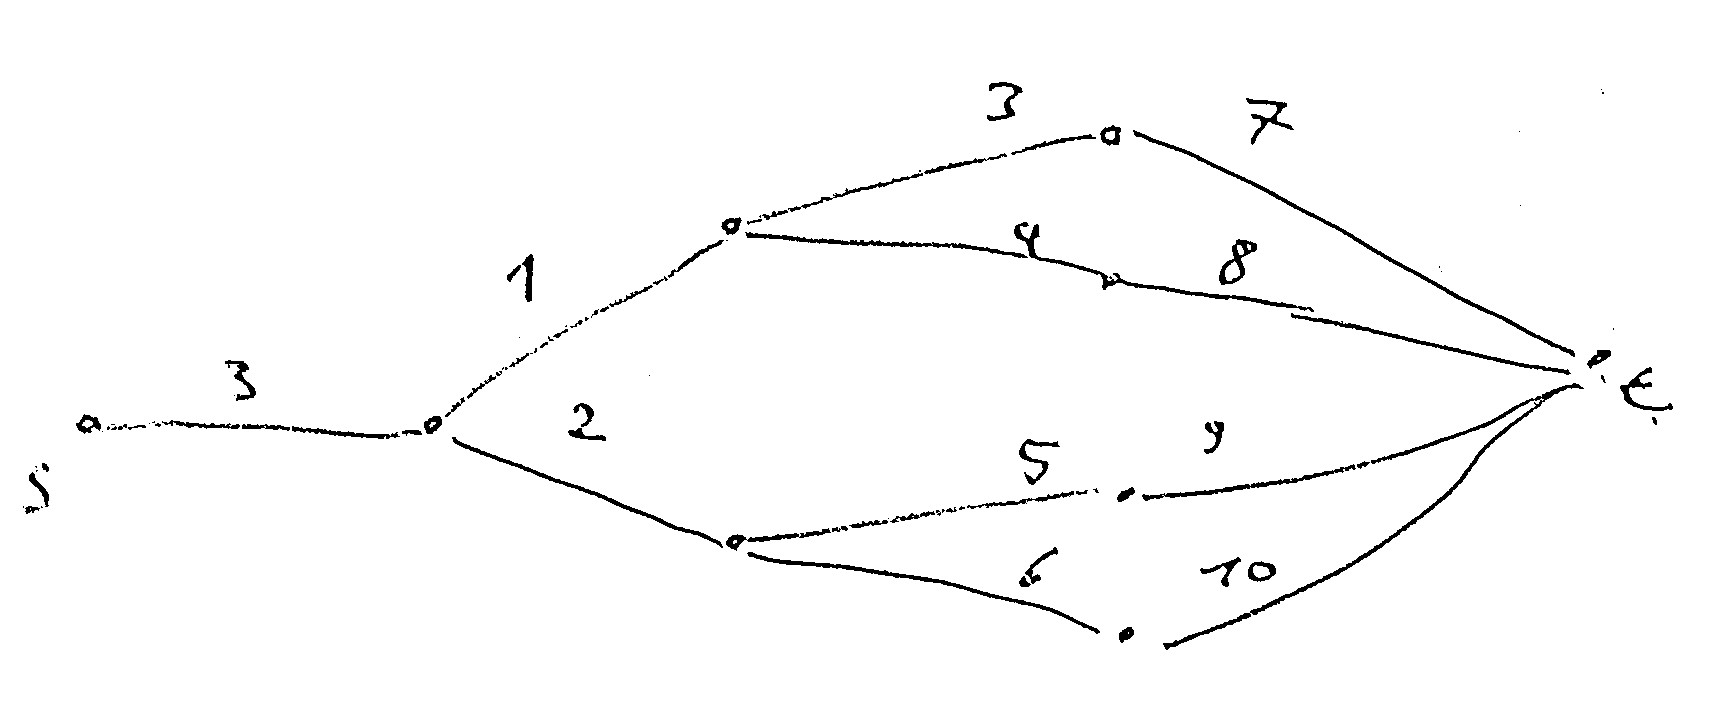
\includegraphics{02_27.jpg}
        }
    \end{figure}
    
\section*{Aufgabe 28}

TODO: buch...

\section*{Aufgabe 29}

    \begin{enumerate}[label={\alph*)}]
        \item \textbf{Max-Flow Min-Cut Theorem:}
            \\ Sei $G=(V,E,c,s,t)$ ein Flussnetzwerk, dann ist der maximale Flusswert in G gleich dem
                minimum der Kapazitäten der s und t separierenden Schnitte. Formal:
                $$
                    \max\{|f| \: |\: f \: \text{ist Fluss in G} \} = \min\{c(S,V \setminus S)\: |\: (S,V \setminus S) \:\text{ist s,t-separierend} \}
                $$
        \item TODO
        \item TODO
  
    \end{enumerate}

\section*{Aufgabe 30}

Wir benötigen noch zusätzlich folgende Definition:
\\ \textbf{Residualgraph: } ein Residualgraph $G_r = (V, E_r)$ von $G$ enthält alle
    Kanten aus $E$ die nicht von f vollständig ausgelastet sind, sowie entsprechende Rückkanten,
    die ``den nicht genutzten Fluss zurückleiten''. Formal bedeutet dies:
    $$
        E_r = \{(v,w) | (v,w) \in E \wedge f((v,w)) < u((v,w))\} \cup \{ (w,v) | (v,w) \in E  \wedge f((v,w)) > 0  \}
    $$
    mit $u_r(e_r), e_r \in E_r$ bezeichnet die Restkapazität einer Kante $e$ wenn $e \in E$,
    bzw. die vom Fluss genutzte Kapazität, wenn $e_r$ eine rückwärtsgerichtete
    Kante zu einer Kante $e \in E$ ist
    Formal:
    $$
        u_r(e_r) :=  \begin{cases}
                            u(e_r ) - f(e_r)  & wenn \: e_r \in E \\
                            f(e_r) & wenn \: e_r^{\leftarrow} \in E
                          \end{cases} 
    $$
    mit $e^{\leftarrow}$ ist Rückwärtskante zu $e$ \\
    
    Der Ford-Fulkerson Algorithmus sucht jetzt quasi nach dem kürzesten Weg
    von s nach t im Residualgraph zu einem Flussnetzwerk G um so 
    den maximalen Fluss in G zu finden.
    \begin{itemize}
        \item \textbf{Eingabe: } Flussnetzwerk $G = (V,E, u,s,t)$
        \item \textbf{Ausgabe: Maximaler Fluss in G} 
        \item \textbf{Methode: } \\
            \begin{algorithm}[H]
                $f(e) := 0$ für alle $e \in E$\;
                \While{$\exists $ Pfad von s nach t in $G_r$}{
                    P := beliebiger Pfad von s nach t in $G_r$\;
                    $\gamma = \min\{u_r(e) | e \in P\}$\;
                    \For{$e \in P \cap E$}{
                        $f(e) := f(e) + \gamma$\;
                    }
                    \For{$e^{\leftarrow} \in P \setminus E$}{
                        $e := (e^{\leftarrow})^{\leftarrow}$\;
                        $f(e) := f(e) - \gamma$\;
                    }
                }
            \end{algorithm}
           (\textbf{Anmerkung:} $G_r$ wird implizit aktualisiert)


    \end{itemize}
    
\section*{Aufgabe 31}

    \begin{enumerate}[label={\alph*)}]
        \item 
            sei n die Summe r Kantenkapaziten in einem Flussnetwerk.
            Dann terminiert Ford-Fulkerson nach maximal n durchläufen.
        \item
    \end{enumerate}


\section*{Aufgabe 32}

    \begin{enumerate}[label={\alph*)}]
        \item \textbf{Algo von Dinic:} \\
            
    \end{enumerate}


\end{document}